\documentclass{article}
\usepackage{listings}
\lstset{
  basicstyle=\ttfamily\scriptsize }
\usepackage{graphicx}
\graphicspath{{.}}
\usepackage{parskip}
\usepackage{amsmath}
\usepackage[margin=2.5cm]{geometry}
\usepackage{hyperref}

% For check marks
\usepackage{tikz} \def\checkmark{\tikz\fill[scale=0.4](0,.35) --
  (.25,0) -- (1,.7) -- (.25,.15) -- cycle;}

% Thanks to Angus Pearson for nagging me to fuck about with fonts in
% XeLaTeX

\usepackage{fontspec} \usepackage{xltxtra}

% PT Serif
\setromanfont[ BoldFont=PTF75F.ttf, ItalicFont=PTZ56F.ttf,
BoldItalicFont=PTF76F.ttf, ]{PTF55F.ttf}

% Noto Sans
\setsansfont[ BoldFont=NotoSans-Bold.ttf,
ItalicFont=NotoSans-Italic.ttf, BoldItalicFont=NotoSans-BoldItalic.ttf
]{NotoSans-Regular.ttf}

\hypersetup{ colorlinks = false }

\begin{document}

\pagestyle{headings}

\textbf{\Huge Computer Security Notes}\\
\textit{\footnotesize Found at: \href{http://benjaminshaw.uk}{benjaminshaw.uk}}

\section{Basics}

\subsection{A Definition of Security}

\textbf{Confidentiality}

Ensure that assets are accessed only by authorised parties.

\textbf{Integrity}

Assets can only be modified by authorised parties, or by authorised
means.

\textbf{Availability}

Assets are only accessible to authorised parties at the appropriate
times.

\textbf{Accountability}

Actions are traceable to those responsible

\textbf{Authentication}

User/data origin accurately identifiable

\subsection{Security Countermeasures}
  
\textbf{Prevention}

Stop security breaches via system design and defences

\textbf{Detection}

If a breach \underline{does} occur, detect it.

\textbf{Response}

A plan utilised when a breach is detected.

\subsection{Denial of Availability}

A user will expect that services be available to them. A common attack
is denying users this privilege. Denial of Service (DOS) attacks or
malware are two common ways of attacking availability.

\filbreak
\section{Cyber Security Essentials}

\subsection{Secure Configuration}

\textbf{Principles:}

Devices on a network should be configured such that they minimise the
number of inherent vulnerabilities.

Default settings can \textit{often} be insecure, which includes
default passwords.

\textbf{Actions:}

\begin{itemize}
\item
  Remove unnecessary user accounts, such as the \textit{Admin}
  account found on Windows XP installs.
\item
  Changing the default password
\item 
  Removal of unnecessary software
\item 
  Firewall software should regulate the incoming/outgoing connections on a device
\end{itemize}

\subsection{Boundary Firewalls \& Internet Gateways}

\textbf{Principles:}

Devices should be protected against unauthorised access and disclosure.

Firewalls are the first line of defence and can stop attacks before they even reach the network.

\textbf{Actions:}

\begin{itemize}
\item 
  Change default passwords
\item 
  Rules should be scrutinised before they are applied
\item 
  Unapproved services should be blocked by a rule
\item 
  Obsolete rules should be purged
\item 
  Firewall administration tools should not be accessible from outwith the network
\end{itemize}

\subsection{Access Control and Privilege Management}

\textbf{Principles:}

User accounts should have the minimum amount of privileges, with extended privileges awarded upon authorisation.

A compromised account with high levels of access can lead to a lot of damage.

\textbf{Actions:}

\begin{itemize}
\item 
  Account creation should be subjected to an approval process
\item 
  Administration accounts should only be used for legitimate administration purposes and \underline{not} activities that can be achieved with a standard account
\item 
  Elevated privilege accounts should require password changes periodically
\item 
  Users should be authenticated before being granted access to devices and applications
\item 
  Elevated accounts should not be used when no longer required
\end{itemize}

\subsection{Patch Management}

\textbf{Principles:}

Remove unnecessary vulnerabilities by keeping software up-to-date.

\textbf{Actions:}

\begin{itemize}
\item 
  Software should be kept up-to-date and fully licenced
\item 
  Out-of-date software removed
\item 
  Updates when made available should be installed in a timely manner
\end{itemize}

\subsection{Malware Protection}

\textbf{Principles:}

Internet-facing devices should make use of malware protection software that continuously monitor for known-malware instances.

\textbf{Actions:}

\begin{itemize}
\item 
  Install anti-malware software
\item 
  Keep said software up-to-date
\item 
  Regularly scan all files
\item 
  Prevent connections to known malicious website
\end{itemize}

\filbreak
\section{Network Security Threats}

\textbf{Types of Threat:}
\begin{itemize}
\item 
  \textbf{Interception}
  \subitem
  Unauthorised viewing of information
\item 
  \textbf{Modification}
  \subitem
  Unauthorised changing of information
\item 
  \textbf{Fabrication}
  \subitem
  Unauthorised creation of information
\item 
  \textbf{Interruption}
  \subitem
  Prevention of authorised access
\end{itemize}

\subsection{Man-in-the-Middle}

When communications between two devices is intercepted and changed by a third party intruder.

Man-in-the-middle is not necessarily an attack, as VPNs are man-in-the-middle by nature.

\subsection{Denial of Service}

When valid users are prevented from accessing a service.

\subsubsection{SYN Flooding}

When a large amount of \textit{SYN requests} are sent to the victim with the intention of overloading them. SYN packets are the first packet sent in a TCP handshake.

The attacker would send many of these packets without acknowledging any of the replies to the point that the receiver can handle no more. 

SYN flooding uses a lot of the attacker's bandwidth, and is also traceable if sent from their own IP. An ideal type of attack against a small target but tends not to be affective against larger targets.

SYN flooding in \textit{conjunction with TCP source spoofing} makes it harder to trace the original attacker and ACKs will be directed to some other address.

\subsubsection{Distributed Denial of Service}

The same concept as a denial of service attack, but multiple systems flood the intended victim.

\subsubsection{Smurfing}

An example of \textit{distributed} denial of service attack.

Exploits the \textit{Internet Control Message Protocol} (ICMP) specification of \textit{pings}, which allow for hosts to indicate that they are alive.

A forged ping packet is constructed with the source IP address as the victim's IP, and is sent to a \textit{smurf amplifier}, subsequently that will swamp the target with replies.

A smurf amplifier is a poorly configured host that will not anticipate this attack, and will reply to the forged host.

\subsection{Domain Name Service Attacks}

Utilising the DNS system, where a DNS record will be maliciously altered to set up a man-in-the-middle attack, or prevent access to some URL.

\filbreak
\section{Network Defences}

\subsection{Firewalls}

Firewalls \textit{divide} the untrusted exterior of the network and the trusted interior of the network; they are said to operate on the \textit{Network} layer, or the 3rd layer, of the IP stack.

Firewalls either run on dedicated hardware or as a software package such as \texttt{iptables}. Hardware firewalls operate faster and act as a physical divider, whereas software is easier to deploy.

Firewalls operate upon a \textit{set of rules}. These rules dictate if it allows or denies any given traffic.

\subsubsection{Packet Filtering}

The simplest task of a firewall, compares packet headers to the pre-defined rules.

However, this does not detect forged packets and requires a large and well-defined set of rules to function well.

\subsubsection{Stateful Inspection}

Remembers state between packets received, unlike a packet filter.

This allows it to filter attacks that utilise the scanning of many ports on a host, as it would detect the high number of packets from one source. With this piece of information, it could add to the firewall rules to block this specific host.

\subsubsection{Application Proxy}

A type of man-in-the-middle attack, as it screens messages received at the \textit{Application} layer of the IP stack.

This allows for the firewall to block application requests, such as emails containing certain words or confidential information from a database leaving the network.

\subsection{Intrusion Detection Systems}

Designed to detect a potential intrusion \textit{in progress}.

IDSs will monitor the network for behaviour similar to that of known attacks and raise the alert when it does so.

There is a fine line to walk as IDS needs to be sensitive to detect attacks, as they are not prone to being as blatant as possible; however, too many false alarms can soon prove to a be a liability.

\subsection{Signature-based}

Utilises \textit{pattern matching}, where a pattern is provided in advance.

This method does not anticipate new types of attack but has a high level of accuracy which is effective for well-known and common types of attack.

\subsection{Heuristic-based}

The method builds a model of what \textit{normal} behaviour looks like. This allows for possible anticipation of new types of attack.

However, it can take a long time to build this model and is susceptible to false positives.

\section{Security Amongst Users}

A large number of attacks occur due to user error, so it is in the best interests of organisations to make sure that users are able to identify attempts to fool them.

\subsection{Phishing Attacks}

A type of attack that \textit{baits} the user into interacting with a malicious object. This can be done by impersonating a person or organisation that the user may trust beforehand.

This type of attack is usually delivered by email to try and get the user to go to an illegitimate link that will provide the user with malware.

\textit{Spear phishing} is used against a small subset of users, but allows for the attacker to craft the attack in a way that is more likely to trick the user.

\textit{Whaling} is an attempt to use a phishing attack against a financially wealthy victim.

Earmarks of a phishing attack are hyper links to an address that is designed to look like something else, e.g. \textit{www.microsoftrewards.legitwebsite.com}, or emails that come with attachments with titles designed to lure the user to open it.

\subsection{SSL/Malware Warnings}

\textit{Secure Socket Layer} is the technology that \texttt{HTTPS} is built upon, and allows for secure communications between two parties.

SSL allows for validation that the two parties are who they say they are and prevents a man-in-the-middle from reading packet contents, as they are encrypted.

Most modern web browsers will alert users when there are \textit{certificate mismatches}, which can be an indication that the website is trying to mimic another's identity.

Many modern browsers will also look up the URL that the user is trying to visit, and cross-reference this with a blacklist of \textit{known malicious websites}. If this check comes back as true, then a warning shall be displayed to users indicating that the site they are trying to visit has been knwon to distribute malicious content.

Whilst this can be effective against users visiting \textit{new} websites, studies have shown that users are likely to ignore such warnings if they are trying to visit a website that they have been to before. This may be because users think that the blacklist check is at error, or that they can trust the source of the link that they are following.

Roughly \textit{one and a half percent} of these warnings are false-positives.

\subsection{Meaningful Warnings}

It is obviously in the best interests of network administrators and developers to have warning messages that are understandable and effective when displayed to a user.

\filbreak
\subsubsection{NEAT}

\begin{itemize}
\item \textbf{Necessary}
  \subitem
  Is there a need for this user to see or decide upon the warning?
\item \textbf{Explained}
  \subitem
  Is all information provided for the user to make an informed decision?
\item \textbf{Actionable}
  \subitem
  Is there a set of steps that the user can take to make the correct decision?
\item \textbf{Tested}
  \subitem
  Have you tested upon someone who would be an expected user, both in benign and malicious situations?
\end{itemize}

\subsubsection{SPRUCE}

\begin{itemize}
\item \textbf{Source}
  \subitem
  Ensure the source of who is asking for the decision is made clear
\item \textbf{Process}
  \subitem
  Provide the user with actionable steps to make a good decision
\item \textbf{Risk}
  \subitem
  Explain the risks of making the wrong decision to the user
\item \textbf{Unique User Knowledge}
  \subitem
  Tell the user the information that \textit{they} bring to the decision
\item \textbf{Choices}
  \subitem
  List available options, \textit{clearly recommending one}
\item \textbf{Evidence}
  \subitem
  Highligh information the user should include or exclude whilst making the decision
\end{itemize}

\section{Overflow Attacks}

\subsection{Vulnerabilities in C}

Many of the original C functions are susceptible to attacks, as they look for the \textit{null byte}, \verb|'\0'|. The attacker can craft an input that doesn't contain the null byte, resulting in the vulnerable code to keep on reading input in. Such fundamentally vulnerable functions are \texttt{strcpy} and \texttt{scanf}.

\filbreak
\subsection{Buffer Overflows}

When executable code is injected into areas of memory earmarked for code execution, by overflowing areas that are, \textit{most likely poorly}, designed to take input.

The malicious code will then be pushed into some other area and possibly change the flow of execution that the program follows.

\subsubsection{Shell Injection}

The aim of this type of attack is to \textit{spawn a shell}, which would give the attacker general access to the victim's system.

\subsection{Integer Overflows}

When an attempt is made to store a value greater than the maximum value an integer can hold.

Poorly implemented code is susceptible to an attack using such a method as it may result in length checks failing to terminate.

\subsection{Formatted String Exploits}

If an attacker is able to ascertain what \textit{format} a program is expecting to receive, they can craft some input that will directly load malicious code into memory.

\subsection{Defences Against Overflow Attacks}

\subsubsection{Stack Canaries}

Named after the canaries used in mines to detect carbon monoxide leaks in deep mines, they are used to detect when an overflow has caused some data within the stack to be overwritten.

The \textit{stack canary} will be placed just before a return pointer. Before execution, the canary will be checked if it still present before the pointer, as to overwrite the pointer, the canary must be overwritten too.

If the canary is not present, the code will not be executed.

Canaries can hold random values calculated at the start of the process, or can hold termination values such as the \texttt{NULL} byte.

\subsubsection{Make Stack and Heap Non-Executable}

Prevention of overflowing code being executed, as the range it is within is not executed. However, the code can still be executed by using some of the \textit{system calls} found within \texttt{libc}.

\subsubsection{Address Space Layout Randomisation}

Standard libraries are placed in randomly allocated, non-standard locations. This prevents attackers from directly pointing to where a system library call may usually be.

\section{Authentication}

To verify a fact about an entity before it can be allowed to execute some action. This can be achieved by requiring something they \textit{know}, \textit{are} or \textit{have}.

\subsection{Multifactor Authentication}

An authentication process that requires more than one factor; examples being the \textit{chip} and \textit{pin} within your bank card.

\subsection{Passwords}

The most popular method of authentication, a \textit{password} is a character string known to the user and system. They are easy to store, enter and require no special equipment whilst being easily scalable.

\subsection{Password Entropy}

The problem is different passwords have differing levels of \textit{safety}.

A bad password would be one that has low \textit{entropy}, or predictable in other words. It is commonly found that users use a common string, such as \texttt{'123456789'}, or an easily identifiable trait about their self, such as their name or date of birth.

A good password contains a wider range of characters, such as special characters and mixed cases.

A way to combat this is utilising \textit{machine generated passwords}. A well made program can create passwords that are much harder to guess, but tend to be harder for a human to remember. Algorithms have been created to create passwords that are \textit{pronounceable}, increasing the likelihood of a human being able to remember it.

\subsection{Protecting Passwords}

Passwords are rendered useless if an attacker is able to compromise the server and learn it that way. There are a number of mechanisms designed to keep passwords safe in the instance that the server has been compromised.

\subsubsection{Hashing}

A \textit{good} hashing function translates some input to some unique output in a way that is hard to determine the underlying function itself.

This means that the server only stores \textit{hashes}, instead of the plain-text passwords. Even if the hashes were obtained, they would be meaningless to the attacker.

A method called \textit{salting} is used as additional input to further increase the security of hashing. This means that for one string as input but a set of different \textit{salts}, the output would be different for each salt.

This can serve as a protection mechanism against \textit{brute force attacks}. If a server is compromised, the attacker could continuously create a number of passwords with the hashing function to figure out the mapping between inputs and outputs. Salting makes this far more difficult to break the hashing function as it would need to be done for \textit{each} salt alongside the hashing function.

\subsubsection{Lockout}

Another brute force attack is to utilise make a massive number of guesses. This takes advantage of the fact that many user-defined passwords are predictable. An attacker can guess many times against an unsecured authentication system and correctly guess the password in a minuscule amount of time if the password has a low enough entropy.

The idea of a \textit{lockout} is to limit the amount guesses that the attacker has before they are prevented from another attempt, or requiring another factor that they may not have.

\subsection{Keys}

Accompanies the concept of using something you \textit{have} as a means of authentication. Like having a key to unlock a physical doors, keys are also used within digital authentication.

\subsubsection{Key Fob}

A \textit{key fob} has a securely generated number that must be provided alongside the password as a means of two factor authentication.

\subsubsection{Public/Private Pair}

A pair of keys, one of which is \textit{private}, the other which is \textit{public}. A message that one locks and the other unlocks, and vice versa.

\subsection{Biometric \& Behaviour}

To accommodate the idea of something you \textit{are} as a method of authentication.

\subsubsection{Fingerprint Readers}

Fingerprints are \textit{nearly unique} to each person, but can sometimes be difficult to read or, more akin to Cold War antics, can be destroyed. They can also never be changed, which is severely detrimental in the event that they are somehow obtained.

\subsubsection{User Behaviour}

A means of \textit{continuous authentication}, a user's behaviour is monitored. A user's typing patterns is something that is hard to mimic, but this can suffer from real world events such as the user being injured.

\section{Access Control}

Governs whether or not some user, (\textit{the principal, or subject}) is allowed access to a resources.

\textit{Information flow control} is a similar concept, but instead scrutinises if an object is allowed \textit{to be known to} a principal.

\subsection{Access Operations}

\textit{Access modes} determine that way that an object can be accessed, with \textit{rights} being a\textit{ combination of such modes}.

\filbreak
\subsubsection{BLP: Bell-LaPadula Model}

A model that enforces confidentiality, it has two access modes: \textit{to observe}, that is examine an object, and \textit{to alter}, that is to change an object.

BLP has the following access rights:

\begin{center}
  \begin{tabular}{|c|c|c|}
    \hline
    & Observe & Alter\\
    \hline
    Execute & & \\
    \hline
    Read & \checkmark & \\
    \hline
    Append & & \checkmark\\
    \hline
    Write & \checkmark & \checkmark\\
    \hline
  \end{tabular}
\end{center}

\subsubsection{Mechanisms for Access Control}

Rights are commonly defined by the \textit{access control matrix} that represents \textit{who} has \textit{which} access to \textit{what}.

There is a set $S$ of objects, a set $A$ of operations that create the matrix $M$.

An example matrix would be:

\begin{center}
  \begin{tabular}{|c|c|c|}
    \hline
    & file1.txt & code.sh\\
    \hline
    User1 & \{\} & \{ \texttt{read} \}\\
    \hline
    User2 & \{ \texttt{read, write, execute}\} & \{ \texttt{read, execute} \}\\
    \hline
  \end{tabular}
\end{center}

\subsubsection{UNIX}

\texttt{UNIX} has three access rights: \texttt{r} for read, \texttt{w} for write, and \texttt{e} for execute.

There are 3 subjects: the \textit{owner}, the \textit{group} and the \textit{world}.

An example of \texttt{UNIX} representing permissions for some file would be:

\texttt{rwxr-----}

The first three characters, \texttt{rwx}, means that the owner can read, write and execute the file. The second, \texttt{r--}, means that the other members of the group can read the file. The final three, \texttt{---}, means that nobody else has any access to the object.

\subsection{Discretionary and Mandatory AC}

\textit{Discretionary} access control means that the \textit{owner} of a resource dictates who may access it, set on a case-by-case basis.

\textit{Mandatory} access control is \textit{system-wide} as per a uniform policy.

\subsection{Multi-Level Security}

A system that has an order of levels, e.g.

\texttt{unclassified $\leq$ confidential $\leq$ secret $\leq$ top secret}

This can express policies meaning that a subject with a slight elevated level of privilege cannot write to an object that has a lower amount required to access it, as this may mean that more privileged information is revealed to those with lower privileges.

But a more flexible policy may be required.

\subsubsection{Security Lattices}

A method of defining a policy of which users can read and write to what levels in a system that utilises multi-level security.

For example, for two subjects \texttt{a} and \texttt{b}, and \texttt{a $\leq$ b}, we would say that b \textbf{dominates} a: \texttt{system low} is the bottom, \textit{dominated} by all others; \texttt{system high} is the top, \textit{dominating} all others.

Say we have two objects that are at differing levels; there is a \textit{minimum} security level for a \textit{subject to access} both.

Now, say we have two subjects that are at differing levels. There is a \textit{maximum} security level for an \textit{object to be} readable by both.


\section{Security on the Web}

The idea is that web-side applications should provide the same guarantee of security as of that of a standalone application.

Visiting a website should not be able to gain local file access, or infect your machine with malware. \textit{Sandboxing} and \textit{privilege separation} act as defences against this.

Nor should one site being accessed compromise connections with other sites; achieved by a \textit{same-origin policy}, isolating one accessed site from others.

\subsection{Injection Attacks}

When malicious information is sent to an \textit{interpreter} that can be executed; subsequently causing damage to the host, or providing information that should not be accessible to the attacker.

\subsubsection{Command Injection}

When a script used by the server reads specially crafted input that is then executed as a system command on the victim's side. This can occur when \textit{data} and \textit{code} share the same channel.

For example, a script may read some input from the user then treats it as directly executable code, which is obviously susceptible to abuse.

Input \textit{validation} and \textit{escaping} serve as defences against this type of injection.

\subsubsection{SQL Injection}

The \textit{Structured Query Language} is the most common language utilised by databases, hence its syntax is well known and used by many, many hosts. A poorly secured host that makes use of a database can be severely damaged if SQL code is injected.

Poorly structured code may take user input and directly feed it to its internal SQL interpreter. The interpreter will execute the code that it is given, which may include more code than the developer intended. 

For example, the website may have a field asking for some text input. If this input is not validated, it could include a command for SQL to delete or return some records, which would will be executed when it is passed along to the interpreter.


\section{Session Hijacking}

\subsection{Cookies and HTTP}

HTTP is a \textit{stateless} system, but can utilise so that a state can be maintained between client and server. There can be difficulties however, as the server may actually be talking to someone who the cookie does not belong to, if the necessary precautions aren't taken.

A unique identifier between the client and the server can be stolen by an attacker; subsequently allowing the attacker to masquerade as the original client to the server.

There are safeguards against this type of theft.

First of all, cookies \textit{tokens} should not be predictable, and tokens should be refreshed periodically.

\subsection{XSS: Cross-Site Scripting}

Many websites make use of client-side scripting languages, such as \textit{JavaScript} as it provides more power to web developers than the markdown languages such as HTML and CSS.

Cross-site scripting is a type of injection attack, where malicious code is inserted into websites that would otherwise be trusted. These sites can then start serving malicious code to unsuspecting users. As the browser on the user's end thinks that the website is trusted, it has no way of knowing that some of the script code being sent from the website is malicious and executes it regardless. This can possibly give the attacker access to session tokens and cookies that belong to other users.

\subsubsection{Reflected XSS}

Where the malicious script is \textit{reflected} off the web server and then delivered over this \textit{presumed to be trusted} route to the victim. The script can be hidden within an error request or search result for example.

\filbreak
\subsection{CSRF: Cross-Site Request Forgery}

When a user is forced to execute unwanted actions on a web application in which they are currently authenticated, attacking requests to change-state rather than stealing data.

This type tries to take advantage of servers that have predictable structures.

The attacker will craft a URL, and then trick the victim to make a request to the vulnerable server. When the victim accesses the malicious URL, the attacker's website will make the victim's browser access the URL that will execute the unwanted action.

CSRF attacks can be prevented by verifying the origin of the request, and not one that has been referred by another website.

\section{Secure Communications}

\textbf{Confidentiality}: Information shouldn't be revealed to unauthorised entities.

\textbf{Authentication}: To know with certainty the entity that you are communicating with.

\textbf{Anonymity}: The identity of the author of an action should not be revealed.

\textbf{Non-Repudiation}: The author of an action should not be able to deny doing so

\textbf{Integrity}: Data should not be altered in an unauthorised manner during creation or transmission.

\textbf{Unlinkability}: An attacker should not be able to see which services have been provided to a user.

\subsection{Cryptography Primitives}

\subsubsection{LFSR: Linear Feedback Shift Register}

A \textit{shift register} that takes its input as the output of the previous sate.

For example, with a 4 bit stream \texttt{1101}, the last two bits would be taken, \texttt{01}. We would then \texttt{XOR} these two bits, which would produce \texttt{1}. This is then placed at the front of the register, shifting the bits currently in the register to the right.

\begin{center}
  \begin{tabular}{c}
    \begin{lstlisting}
      0 XOR 1 = 1
      -----------
       1 -> 1101
       1110 -> 1   # this bit is popped
                   off of the register
    \end{lstlisting}
  \end{tabular}
\end{center}

\filbreak
\subsubsection{CSS: Content Scrambling System}

Makes use of \textit{LFSR} with a key size of 40 bits, used on \textit{DVD-Video}.

\textbf{Initialisation:}

A 17-bit LSFR is initialised as the concatenation of 1 and the first 16 bits of the key.

A second, 25-bit LSFR is initialised as the concatenation of 1 and the remaining 24 bits of the key,

\textbf{Action:}

We take the sum of the output of two LSFRs plus any remainder from the previous, modulo 256. This produces a byte of output.

\textbf{Flaws:}

As the video encoding used in DVD-Video is \textit{MPEG-2}, of which the first 290 bytes are plain text. This means that we know the first 20 bytes of the keystream.

Through brute force on the 17-bit LSFR, of which there are $2^{17}$ possibilities, we can deduce the output of the 25-bit LSFR using subtraction.

\subsection{Perfect Secrecy}

A cipher satisfies \textit{perfect secrecy} if, for all messages of the same length, for all encrypted messages:

\[ | Pr(E(k, m_1) = c) - Pr(E(k, m_2) = c) | \leq \epsilon \]

In plain English, absolutely no information about the unencrypted message will be revealed by the encrypted message.

\filbreak
\subsection{Symmetric Ciphers}

For some message, you have an encryption algorithm, $E$, and a decryption algorithm, $D$, such that:
\vspace{.5cm}
\begin{center}
  $K$ is some secret key known between the two parties\\
  $C$ is the encrypted message
  $M$ is the unencrypted message
\end{center}

\[ E : K \times M \rightarrow C\]
\[ D : K \times C \rightarrow M\]

Examples include one-time pads, \texttt{DES} and \texttt{AES}.

\subsubsection{OTP: One-Time Pad}

Assumes that the message, encrypted message, and key are all of the same length.

Either the message or encrypted message, and the key, will be \texttt{XOR}'d to produce the desired output.

\begin{figure}[!htb]
  \begin{minipage}{0.5\textwidth}
    \begin{tabular}{c}
      \textbf{Encryption}
      \begin{lstlisting}
        k | 0 1 1 0 1 0 0 1
        m | 1 0 0 0 1 0 1 1
        -   - - - - - - - -
        c | 1 1 1 0 0 0 1 0
      \end{lstlisting}
    \end{tabular}
  \end{minipage}%
  \begin{minipage}{0.5\textwidth}
    \begin{tabular}{c}
      \textbf{Decryption}
      \begin{lstlisting}
        k | 0 1 1 0 1 0 0 1
        c | 1 1 1 0 0 0 1 0
        -   - - - - - - - -
        m | 1 0 0 0 1 0 1 1
      \end{lstlisting}
    \end{tabular}
  \end{minipage}%
\end{figure}

Drawbacks of the OTP is that they key \textit{must} be the same length as that of the message, and that OTPs do not guarantee \textit{true} randomness.

\subsubsection{Stream Cipher}

Similar to the One-Time Pad, but instead of using a really random key, a \textit{psuedo-random} key is used. That is, a key that \textit{looks} random, but is not random in reality.

The stream cipher functions in a way similar to that of the one-time pad, but can utilise a more convenient key which can differ in length from that of the message.

\newpage
\textbf{\underline{RC4}}

A stream cipher used by \textit{HTTPS} and \textit{WEP}.

RC4 consists of two parts: the \textit{Key-Scheduling Algorithm}, and the \textit{Pseudo-Random Generation Algorithm}.

\textbf{Key-Scheduling Algorithm:}

The \textit{KSA} makes use of a \textit{secret key} of a variable length; using it in conjunction with an ordered array of 256 elements, $S$. The aim is to make the array \textit{look} like it has been randomly ordered. After this has been done, the algorithm moves onto the next step.

\textbf{Psuedo-Random Generation Algorithm:}

The \textit{PRGA} increments over the message \underline{and} outputs one byte at a time.

\begin{lstlisting}[language=C]
  i := 0; j := 0;
  do{
    i := (i + 1) mod 256;
    j := (j + S[i]) mod 256;
    swap(S[i], S[j]);
    K := S[(S[i] + S[j]) mod 256];
    output K;
  }while(required);
\end{lstlisting}

So, we have an element of $S$, found at index $i$, which is swapped with another element of $S$, at index $j$. These two elements are summed, with the result \textit{modulo 256} which gives us the next element of the \textit{resulting encrypted array}. At each iteration, we recalculate $i$ and $j$:
\[ i = (i + 1)\:\text{mod}\:256\]
\[ j = (S[i] + S[j])\:\text{mod}\:256\]

The number of iterations is equal to the length of the \textit{key}.

\subsubsection{Block Ciphers}

A \textit{deterministic algorithm} that operate on fixed-length \textit{blocks} of bits.

The block cipher will take some size bit of plain text, and output the same size of cipher text. A \textit{key} is used to determine the exact transformation between plain and cipher text.
\newpage
\textbf{\underline{DES: Data Encryption Standard}}

An primitive version of the block cipher that found widespread use after being developed in the 1970s.

\textit{DES} takes a block of size 64 bits from the plaintext, and uses a key of size 64 bits\footnote{DES only makes use of 56 bits of the key, the remaining 8 bits are used to check parity (a check bit)}. The output generated is of size 64 bits.

First, the plain text block is taken in and its order of contents changed.

Second, this transformed plaintext is fed through 16 \textit{submodules}; each submodule takes in a different permutation of size 48 bits, from the key.

Third, each submodule has the same combination of operations that permute its input with the given key, which is then \texttt{XOR}'d with the key and then fed to the next module.

Finally, the ciphertext is transformed once again, in a fashion similar to the first step, and produces the ciphertext output.

It is the same process to decrypt the ciphertext if in possession of the key. Providing DES with the ciphertext and they key will produce the plaintext as output.

\textit{However}, DES is susceptible to brute force attacks. An \textit{exhaustive search}, over the key space, can be completed in $2^{56}$ time.

\textbf{\underline{AES: Advanced Encryption Standard}}

Intended as the successor to DES.

Makes use of a block size of 128 bits, and the key size is either 128, 192 or 256 bits.

\subsubsection{Using Block Ciphers}

Block ciphers offer different \textit{modes of operation}, which define the fundamental behaviour of the block cipher.

\textbf{\underline{ECB: Electronic Code Book}}

The message $M$ is divided into blocks, with each block being encrypted with key $K$ separately. No interaction takes place between each block being encrypted.

The main issue with this method is that it doesn't hide \textit{patterns} well at all, as identical plaintext blocks produce identical ciphertext blocks.

\begin{figure}[htb!]
  \begin{minipage}{0.5\linewidth}
    \centering
    
\includegraphics[scale=0.4]{tux.jpg}\\
    \textit{Before encryption}
  \end{minipage}
  \begin{minipage}{0.5\linewidth}
    \centering
    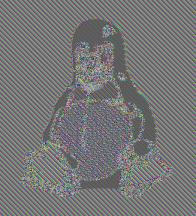
\includegraphics[scale=0.4]{tuxecb.jpg}\\
    \textit{After encryption using ECB}
  \end{minipage}
\end{figure}

\newpage
\textbf{\underline{CBC: Cipher Block Chaining}}

Introduces the \textit{initialisation vector}.

The first block and the IV are \texttt{XOR}'d, then fed to the block cipher with a key $K$, producing the first block of the ciphertext.

This block of ciphertext is then \texttt{XOR}'d with the next block of plain text, and once again fed to the block cipher. This continue is represented until the final block of cipher text is created.

The downside of this is that encryption must be sequential.

\textbf{\underline{CTR: Counter}}

Turns a block cipher \textit{into a stream cipher}.

CTR makes use of a function that produces \textit{successive values} which are then fed to the cipher, \texttt{XOR}'d with the plaintext which produces the ciphertext.

\subsection{Asymmetric Ciphers}

For some message, you have a key generation algorithm, $G$, as well as
encryption and decryption algorithms, $E$ and $D$ respectively.

\vspace{.5cm}
\begin{center}
  $K$ is some secret key known between the two parties\\
  $C$ is the encrypted message $M$ is the unencrypted message
\end{center}

\[ E : K \times M \rightarrow C\]
\[ D : K \times C \rightarrow M\]
\[ G : K \times K \]

The decryption key is secret, or \textit{private}, whereas the
encryption key is \textit{public}.

An example would be \texttt{RSA}.
 
There is also use for \textit{digital signatures}, which is the
production of another key, the \textit{verification key}, which is
know to everyone but differs from the signing key. This can deduct
whether or not some message has been encrypted under some given key.

\filbreak
\subsubsection{Establishing a Secret Key}

\textbf{\underline{TTP: Trusted Third Party}}

Users establish their key with a third party that they both trust.

Lets say we have two parties, $A$ and $B$ with the trusted third party $S$.

$A$ sends their key, encrypted under $K_{AS}$ to $B$.

$B$ receives the message, attaches their own key encrypted under $K_{BS}$ and sends it to $S$.

$S$ creates the key $K_{AB}$, sends it to $A$ under the key $K_{AS}$. Also within this message is they key required for $B$, under the key $K_{BS}$, which $A$ forwards to $B$.

\textbf{\underline{Public-Private Pair}}

Lets say $A$ wants to send a message to $B$

$B$ sends some key that $A$ will encrypt the message under.

$A$ encrypts the message using that key, and then sends it to $B$.

$B$ receives the message and unlocks it with a decryption key - known \textit{only} to him.

\textbf{\underline{D-H: Diffie-Hellman Protocol}}

First, we must understand we must understand two concepts to use this protocol.

The \textit{discrete logarithm}, and the \textit{primitive root modulo}.

\fbox{%
  \begin{minipage}{1.0\textwidth}
    \textit{\underline{Primitive Root Modulo}}
    
    We say a number $g$ is primitive root modulo $n$ if \underline{every} \textit{coprime} of $n$ is congruent to $g$ modulo $n$.
  \end{minipage}
}

\fbox{
  \parbox{\textwidth}{%
    \textit{\underline{Discrete Logarithm}}
    
    For an equation of the form $b^k = g$, we say $k$ is a discrete logarithm.
    }%
}

So, $A$ and $B$ agree to use a modulus $p$, and base $g$ (which is a primitive root modulo of $p$).

$A$ then chooses a secret integer, $a$, and sends $B$:

\[ A = g^a \text{ mod } p\]

$B$ then chooses a secret integer, $b$ and sends $A$:
\[ B = g^b \text{ mod } 23\]

$A$ and $B$ compute $s$ with the message they were sent.

\[ \text{A computes: } s = B^a \text{ mod } p \]
\[ \text{B computes: } s = A^b \text{ mod } p \]

$A$ and $B$ will have both arrived at the same value $s$ under mod $p$.

\subsection{Hashes}

An algorithm $H$, that takes a message $M$ and produces a unique hash value $D$, such that:

\[ H : M \rightarrow D\]

Hashing algorithms should be \textit{pre-image resistant}, where it should be impossible to take the output of the hashing function and determine the original message fed to the function. There should also be \textit{collision resistance}, where it should be extremely difficult to have two different messages produce the same hash.

Hashing function examples would be \texttt{MD5} and \texttt{SHA-1}.

\subsection{OWF: One-Way Functions}

A function $f$ is one-way if there is no efficient algorithm that can compute the function's domain given its co-domain.

The multiplication of two different primes is an OWF, but the successor function is not an OWF.

\subsection{CRF: Collision-Resistant Functions}

A function $f$ is collision resistant if there is no efficient algorithm that can find two messages, $m_1, m_2$ where $f(m_1) = f(m_2)$.

\subsection{Hashing Function}

A \textit{cryptographic hash function} $H : M \rightarrow T$ must satisfy four properties:

\begin{itemize}
\item
  $|M| > |T|$
\item
  easy to compute has for any given message
\item
  hard to retrieve a message from its hashed value (OWF)
\item
  hard to find two different messages with the same hash value (CRF)  
\end{itemize}

Hashing functions allow for participants to commit to some \textit{hashed} value without revealing the original message, useful for electronic voting. Also useful for verifying integrity of a file or password.

\subsection{MAC: Message Authentication Codes}

A short piece of information that is used to \textit{authenticate} a message.

A MAC function take a key and a message as input, and outputs a \textit{MAC tag}. The value protects both \textit{integrity} and \textit{authenticity} of the message, as any changes to the content are detected.

\begin{appendix}

\end{appendix}

\section{Representing the Stack}

\subsection{Register Values}

\begin{tabular}{|c|l|}
  \hline
  \texttt{\%ebp} & Base\\
  \hline
  \texttt{\%esp} & Stack Frame\\
  \hline
  \texttt{\%eip} & Instruction\\
  \hline
  \texttt{\%eax} & Return Value\\
  \hline
\end{tabular}

\subsection{Example}

\textbf{Code:}
\begin{lstlisting}[basicstyle=\ttfamily]
  main{
      f(arg1, arg2);
      b = a;
  }

  f(arg1, arg2){
      return arg1 + arg2;
  }
\end{lstlisting}

\textbf{Process:}
\begin{enumerate}
\item
  Push arguments onto stack (in reverse)
\item
  Push return address
\item
  Jump to function address
\item
  Push old frame pointer onto the stack: \texttt{\%ebp}
\item
  Set frame pointer to where the end of the stack is: \texttt{\%esp}
\item
  Push local variables onto the stack
\item
  Reset previous stack frame
\item
  Jump back to return address

\end{enumerate}

\end{document}
